\section{Resultados}

\subsection{Casos de experimentación}

Nuestras experimentaciones revuelven sobre tres experimentos distintos:
\begin{itemize}
	\item Dadas una altura y número de secciones fijas, y una carga constante distribuida uniformemente sobre el puente, variar el \textit{span} del puente, y analizar el comportamiento de las fuerzas máximas.
	\item Repetir el experimento anterior pero con el mismo peso total de cargas situado en el centro del puente.
	\item Dado un \textit{span} y altura fijos, y un peso total distribuido uniformemente, estudiar el efecto de subdividir el puente en más o menos juntas.
	\item Adicionalmente, analizar si posicionar una carga asimétricamente en el puente genera comportamientos interesantes.
\end {itemize}

En todos los casos, concentramos nuestros estudios en el valor absoluto de la máxima fuerza ejercida, y en la distribución de fuerzas ejercidas en todos los links, discriminadas por la clase de link.\\

Si bien teóricamente los resultados deberian ser siempre idénticos en los links
que se reflejan simétricamente, pequeñas diferencias debido a la imprecisión
numérica del algoritmo hacen que esto no siempre sea el caso. No obstante,
en ninguna observación de cualquiera de los experimentos hubieron discrepancias
por encima del $1\%$ del mejor resultado obtenido por el \textit{solver} de \textit{NumPy}.\\

\subsection{Experimento 1: Aumentar el span con carga uniforme}

Para este tipo de experimento fijamos todos los parámetros e incrementamos el $span$. El propósito de esta prueba era observar como iba evolucionando la fuerza máxima aplicada en los links.\\

Mostraremos dos gráficos en los cuales el set de datos será \textit{span: 8},
\textit{altura: 3}, y \textit{carga por sección: 5} para $i \in [1 \dots 7]$ en el primer gráfico y
\textit{span: 20}, \textit{altura: 3} y \textit{carga por sección: 5} para $i \in [1 \dots 19]$ para el segundo.\\

Nuestra hipótesis es que las fuerzas irían aumentando a medida que el $span$
aumenta, ya que la longitud por cada sección aumentahaciendo que los links tengan que soportar más peso. Veamos lo que realmente sucede.\\



\begin{figure}[h!]
	\begin{center}
	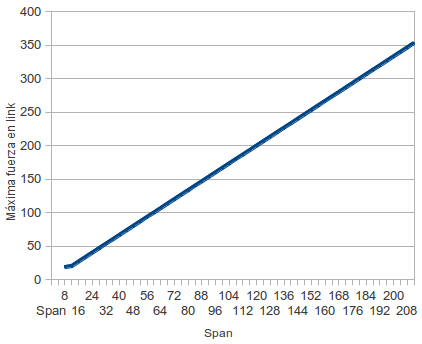
\includegraphics[scale=0.8]{archivos/graficos/Fuerza-x-span.png}
	\caption{\label{fig:fuerza_x_span}Fuerza máxima por Span de puente\\  \textit{Secciones}: $8$, \textit{altura}: $3$, \textit{peso de cargas}: $5$}
	\end{center}
\end{figure}

\begin{figure}[h!]
	\begin{center}
	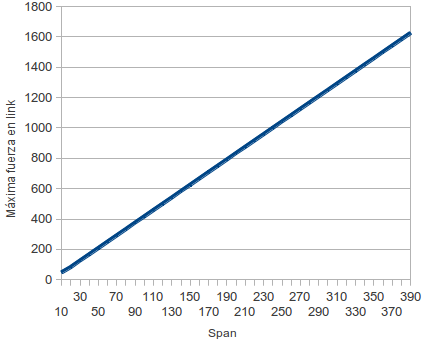
\includegraphics[scale=0.8]{archivos/graficos/Fuerza-x-span2.png}
	\caption{\label{fig:fuerza_x_span2}Fuerza máxima por Span de puente\\  		\textit{Secciones}: $8$, \textit{altura}: $3$, \textit{peso de cargas}: $5$}
	\end{center}
\end{figure}

En las figuras \ref{fig:fuerza_x_span} y \ref{fig:fuerza_x_span2}, podemos observar que la máxima fuerza en algún link del puente crece linealmente conforme aumenta el $span$. Es interesante notar que en los primeros dos casos, donde el ratio de \textit{ancho vs. altura} no supera $0,5$ la máxima fuerza es la compresión que reciben los links diagonales de los extremos, que soportan el peso completo del puente. De ahi en adelante la máxima fuerza es la compresión sufrida por los links centrales superiores.\\

Conforme las secciones del puente se hacen más anchas, esa carga aumenta linealmente, indicando que estas vigas soportan el mayor nivel de compresión y fuerza, y el análisis de costo de un puente deberia tomar este hecho en cuenta.\\

\subsubsection{Distribución de la cantidad de fuerzas}

Analicemos ahora la distribución de la cantidad de fuerzas en los casos cuando el \textit{span} es $200$ y $400$. En la figura \ref{fig:hist_fuerzas} el set de datos será: \textit{segmentos: 20}, \textit{altura: 3} y \textit{carga por sección: 5} para $i \in [1 \dots 19]$, y en \ref{fig:hist_fuerzas2}, observamos el comportamiento de un puento con la misma altura y peso, pero dos veces más largo.

\begin{figure}[h!]
\begin{center}
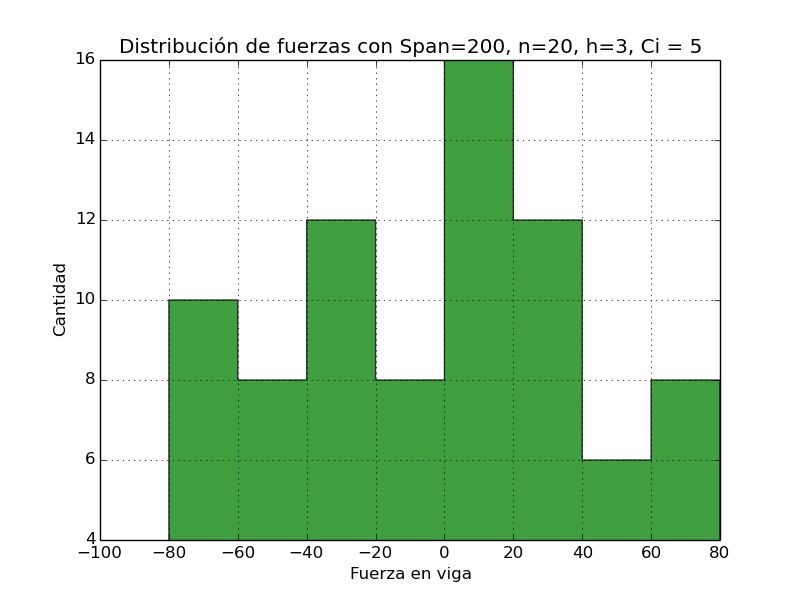
\includegraphics[scale=0.5]{archivos/graficos/hist_200.png}
\caption{\label{fig:hist_fuerzas}Histograma de distribución de fuerzas\\
\textit{Span}: $200$, $n$: $20$, $h$: $3$, $C_i$: $5$}
\end{center}
\end{figure}

\begin{figure}[h!]
\begin{center}
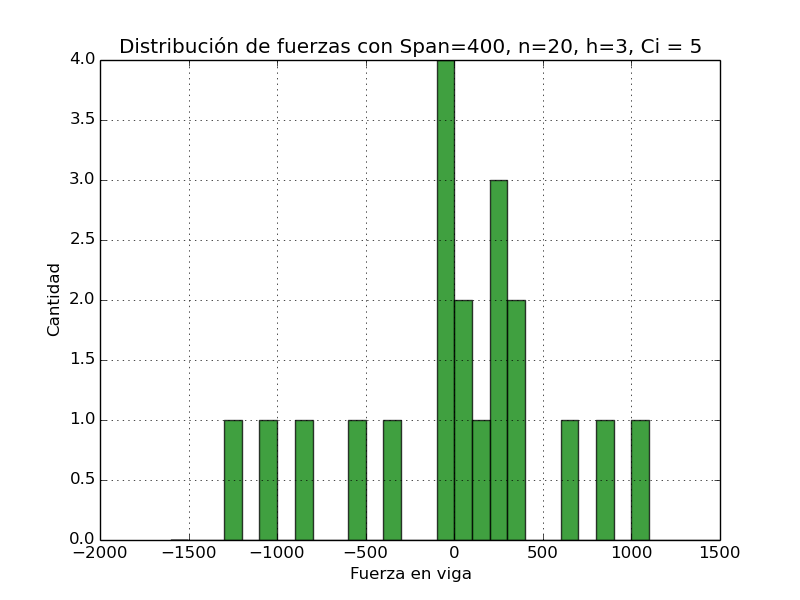
\includegraphics[scale=0.5]{archivos/graficos/hist_400.png}\\
\caption{\label{fig:hist_fuerzas2}Histograma de distribución de fuerzas\\
\textit{Span}: $400$, $n$: $20$, $h$: $3$, $C_i$: $5$}
\end{center}
\end{figure}

Comparando ambos gráficos se puede ver que la fuerza de las juntas se concentra
en la cercanía a $0$, y luego las fuerzas se distribuyen uniformemente hacia los extremos. Analizando los resultados emitidos por el programa, resulta que los links verticales y diagonales son los que suelen sufrir las menores fuerzas, y el grueso de las fuerzas internas afectan a los segmentos horizontales.

Es interesante notar que la distribución de fuerzas es similar en ambos casos; lo único que cambia es la magnitud de las fuerzas, que, como vimos en \ref{fig:fuerza_x_span} y \ref{fig:fuerza_x_span2}, incrementa linealmente.

\subsection{Experimento 2: Aumentar el span, pero fijando una carga central}

Ahora veamos qué sucede cuando aumentamos el $span$, dejando todo fijo pero
 colocando solamente un peso significativo en la junta central y fijando las restantes en $0$.\\

\begin{figure}[h!]
\begin{center}
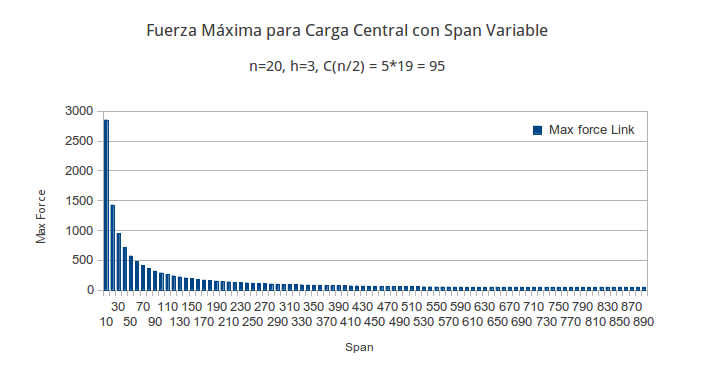
\includegraphics[scale=0.8]{archivos/graficos/Fuerza-x-span-peso-central.png}
\caption{\label{fig:fuerza_x_span_peso_central}Fuerza máxima por Span de puente con carga central\\
\textit{Secciones}: $20$, \textit{altura}: $3$, \textit{peso total}: $5 * 19 = 95$}
\end{center}
\end{figure}

Cuando ponemos el peso equivalente a la carga distribuida uniformemente en el
vértice central, notamos que el comportamiento es idéntico al experimento
anterior en forma, pero la fuerza máxima soportada por un link es considerablemente mayor, y el valor del span desde el cual la fuerza máxima es soportada por los links diagonales exteriores es mayor (cuando $span = 600$).\\

Esto se explicaría porque la distribución centralizada del peso fuerza a que los links centrales concentres las fuerzas de la carga sin la ayuda de los links más distantes del centro del puente, que juegan un mayor rol cuando el peso es más uniforme.

\newpage
\subsection{Experimento 3: Cambiar la cantidad de secciones}

Ahora analizamos cómo se comportan las fuerzas de los links cuando cambiamos la cantidad de secciones en los que está subdividido.\\

En las figuras \ref{fig:hist_n100_C100} y \ref{fig:hist_n10_C100}, generamos un puente de longitud $100$, con el primer caso teniendo $100$ secciones, y en el segundo caso, solo $10$.

\begin{figure}[h!]
\begin{center}
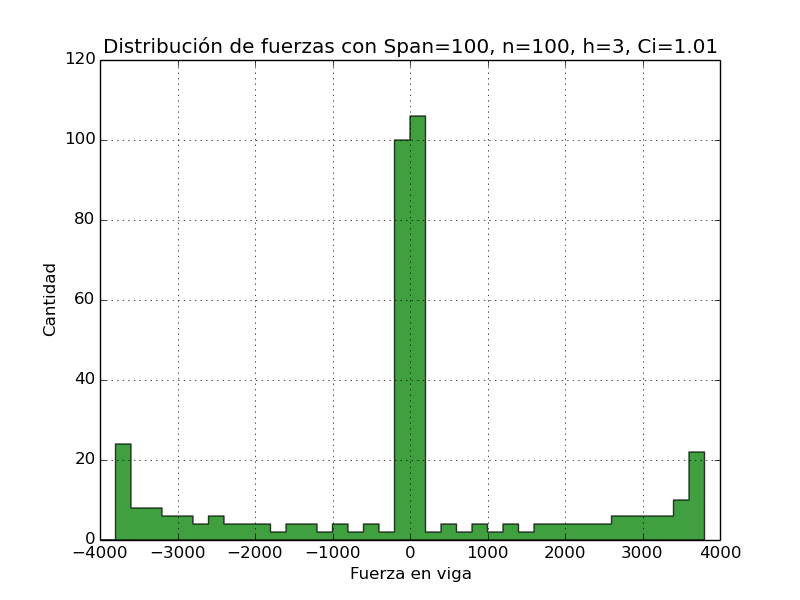
\includegraphics[scale=0.5]{archivos/graficos/hist_n100_C100.png}
\caption{\label{fig:hist_n100_C100}Histograma de distribución de fuerzas\\
\textit{span}=$100$, $n=100$, $h=3$, $C_i=1,01$}
\end{center}
\end{figure}

\begin{figure}[h!]
\begin{center}
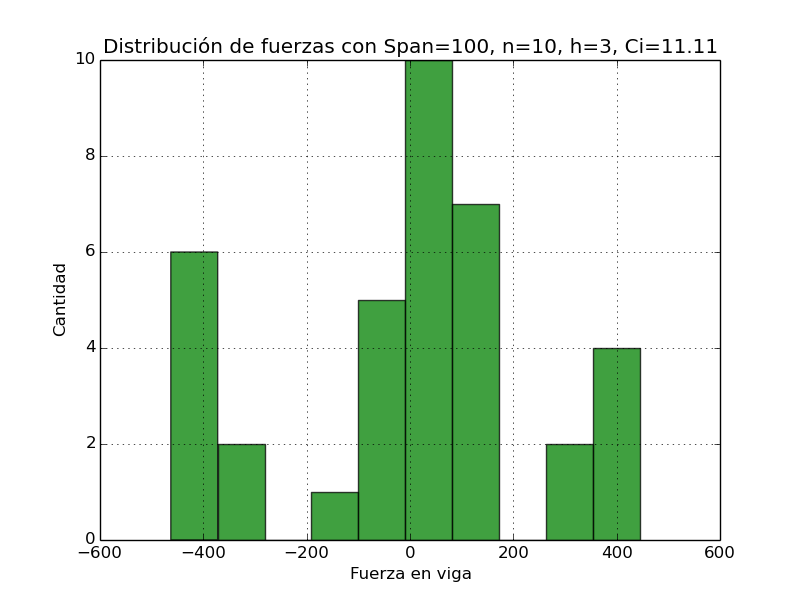
\includegraphics[scale=0.5]{archivos/graficos/hist_n10_C100.png}
\caption{\label{fig:hist_n10_C100}Histograma de distribución de fuerzas\\
\textit{span}=$100$, $n=10$, $h=3$, $C_i=11,11$}
\end{center}
\end{figure}

\begin{figure}[h!]
\begin{center}
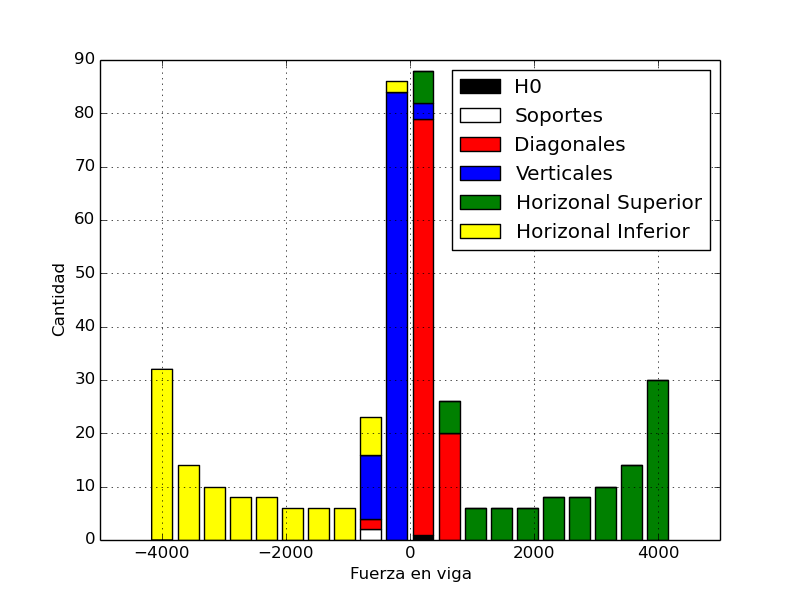
\includegraphics[scale=0.5]{archivos/graficos/hist_n100_C1000.png}
\caption{\label{fig:hist_n100_C1000}Histograma de distribución de fuerzas\\
\textit{span}=$100$, $n=100$, $h=3$, $C_i=10,10$}
\end{center}
\end{figure}

\begin{figure}[h!]
\begin{center}
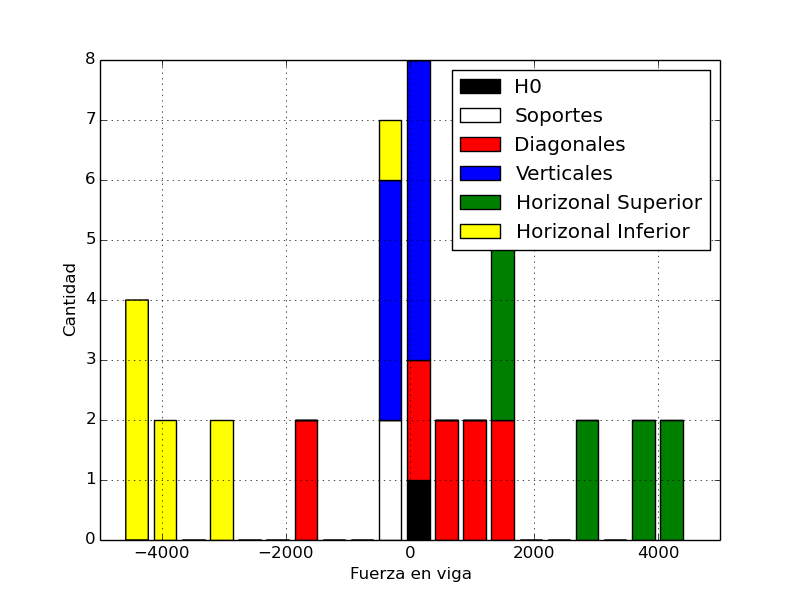
\includegraphics[scale=0.5]{archivos/graficos/hist_n10_C1000.png}
\caption{\label{fig:hist_n10_C1000}Histograma de distribución de fuerzas\\
\textit{span}=$100$, $n=10$, $h=3$, $C_i=111.11$}
\end{center}
\end{figure}

Observamos que la máxima fuerza en los puentes densos y esparsos de misma longitud son similares, con el puente con menos links teniendo, en proporción levemente más links en los extremos, y las diagonales soportando un poco más de carga, aunque igualmente más cerca del cero que de los valores extremos.\\

Nótese que en el caso donde \textit{span}$=100$ y $n=10$, cada sección tiene una longitud de $10$ y altura de $3$ (es decir, es más ancha que alta), y cuando \textit{span}$=100$ y $h=100$, las mismas son rectangulares pero más altas que anchas.\\

Desde un punto de vista de costo y eficiencia en términos de utilización de material, la opción de usar menos links y tener secciones más anchas resulta preferible por sobre la inversa.\\

\subsubsection{Estudio con cargas asimétricas}
Probamos también aumentar el \textit{span} con carga asimétrica con \textit{número de secciones} $=20$, poniendo pesos en los links inferiores de las secciones $4$ y $5$. Observamos que el comportamiento sigue siendo el mismo que en las figuras anteriores (es decir, una fuerza máxima grande que aumenta linealmente sobre el \textit{span}) relativo a la fuerza máxima, salvo que la misma ahora está situada en las secciones superiores directamente encima de los pesos.\\

Esto se explica debido a que los pesos flexionan el puente hacia abajo, y por ende los links superiores a los pesos sufren un efecto de compresión que permite que la estructura permanezca estable. Dado que en esta prueba el único cambio sobre las anteriores es que el peso está distribuido asimétricamente y en forma concentrada, es razonable que la estructura se siga comportando físicamente con el mismo patrón.\\

La figura \ref{fig:hist_asim} muestra la distribución de fuerzas en los links discriminada por tipo de link. Tal como analizamos en casos anteriores, las fuerzas diagonales y verticales son relativamente bajas en el espectro total, mientras que los extremos son dominados por las fuerzas horizontales, con las superiores sufriendo compresión, y las inferiores, tensión.

\begin{figure}[h!]
\begin{center}
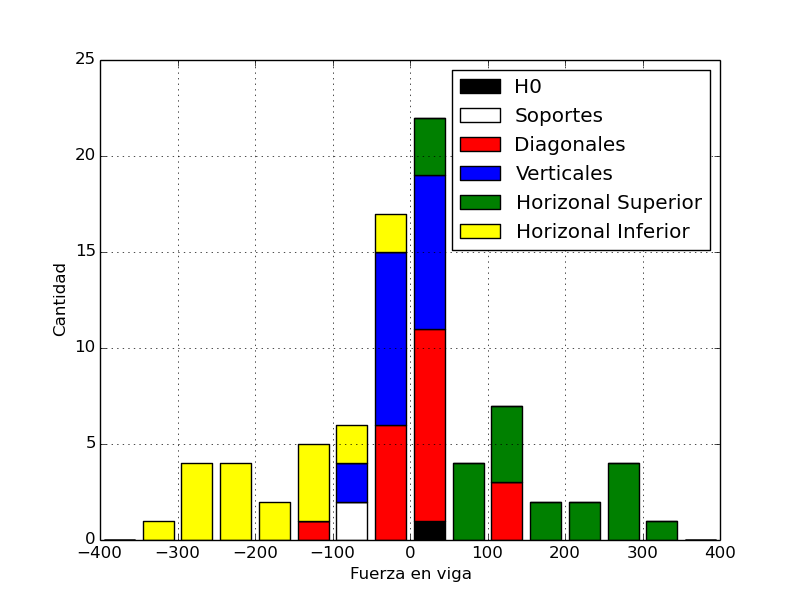
\includegraphics[scale=0.5]{archivos/graficos/hist_asim.png}
\caption{\label{fig:hist_asim}Detalle de distribución de fuerzas\\
\textit{span}=$60$, $n=10$, $h=3$, $C_i$ \textit{asimétrico}}
\end{center}
\end{figure}


